\documentclass[crop,tikz]{standalone}

\usetikzlibrary{positioning}
\usepackage[utf8]{inputenc}

% 'crop' is the default for v1.0, before it was 'preview'
%\usetikzlibrary{...}% tikz package already loaded by 'tikz' option
\usetikzlibrary{arrows} 

\begin{document}

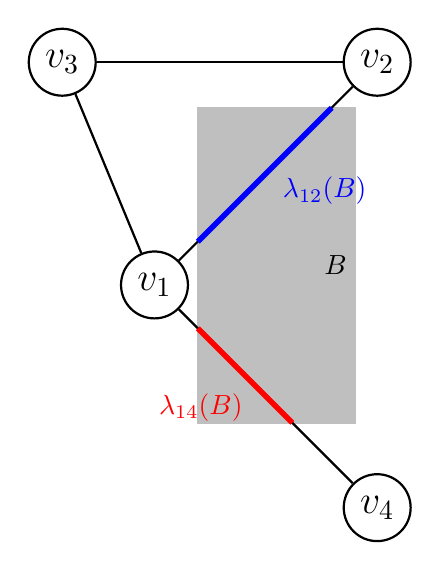
\begin{tikzpicture}[-,>=stealth',auto,node distance=4cm,thick,main node/.style={circle,draw,font=\sffamily\Large\bfseries}]

	%draw a "set" in 2D space that covers some of the lines
	\begin{scope}[scale=1.0, shift={(0.55,-1.75)}]
		\filldraw[color=black!50!white!50!] (0,0) rectangle (2,4);
		\node at (1.75,2) {$B$};
	\end{scope}

	%some graph to act as the background for illustrating the measure properties	
	\begin{scope}
		\node[main node] (1) {$v_{1}$};
		\node[main node] (2) [above right of = 1] {$v_2$};
		\node[main node] (3) [left of = 2] {$v_3$};
		\node[main node] (4) [below right of = 1] {$v_4$};
		
		\path[every node/.style={font=\sffamily\small}]
			(1) edge (2)
			(2) edge (3)
			(1) edge (4)
			(1) edge (3);
	\end{scope}
	
	%finally, draw the edge measures and the sets they care about
	\begin{scope}
		\draw[red, line width=2] (0.55,-0.55) -- (1.75,-1.75);
		\node[red, anchor=north east] at (1.25,-1.25) {$\lambda_{14}(B)$};
		
		\draw[blue, line width=2] (0.55, 0.55) -- (2.25,2.25);
		\node[blue, anchor=north west] at (1.5,1.5) {$\lambda_{12}(B)$};
	\end{scope}
\end{tikzpicture}

\end{document}